

\chapter{Podstawy teoretyczne}
\label{cha:podstawyTeoretyczne}

\section{Rodzaje map}
\label{sec:Rodzaje map}

Tworząc aplikację która ma dostarczać informacji korzystających z map należy zapoznać się dostępnymi źródłami. Z powodu szrokiego wyboru poniżej omówione zostaną jedynie aplikacje które dostarczają informacji ogólnoświatowych. Na rynku dostępnych jest kilka rozwiązań polskich, ich główną wadą jest ograniczenie do terytorium Polski, dodatkowo często nie dostarczają one obrazów satelitarnych, są to m.in. \underline{\texttt{http://zumi.pl}}


\subsection{Google Maps}
\label{subsec:Google Maps}
\nocite{googlemapsbegin}
Rysunek \ref{fig:googleMaps_1} przedstawia obraz otrzymany w aplikacji Google Maps. Dodatkowo włączona opcja prezentacji natężenia ruchu jedynie potwierdza duże możliwości i łatwość obsługi. Przyjazny interfejs sprawia że praca jest prosta i pozwala na osiągnięcie bardzo dobrych wyników.

Podczas badań literaturwoych nie odnaleziono oficjalnych danych dotyczących wielkości wykorzystywanej bazy danych.
Natknięto się natomiast na wiele dyskusji i spekulacji, niektóre zawierały przybliżone obliczenia które pozwalają ocenić wielkość bazy danych używanej jedynie dla potrzeb map dochodzącej do 1PB(1024TB czyli 10 do 15 bajtów).
Jest to wiarygodna wielkość w sytuacji gdy oficjalne stnowisko rzecznika prasowego mówi o 20 PB przypadających na wszystkie usługi zdjęc ziemi i widoku z ulicy.\cite{googledatabase}


\begin{figure}[H]
  \centering
    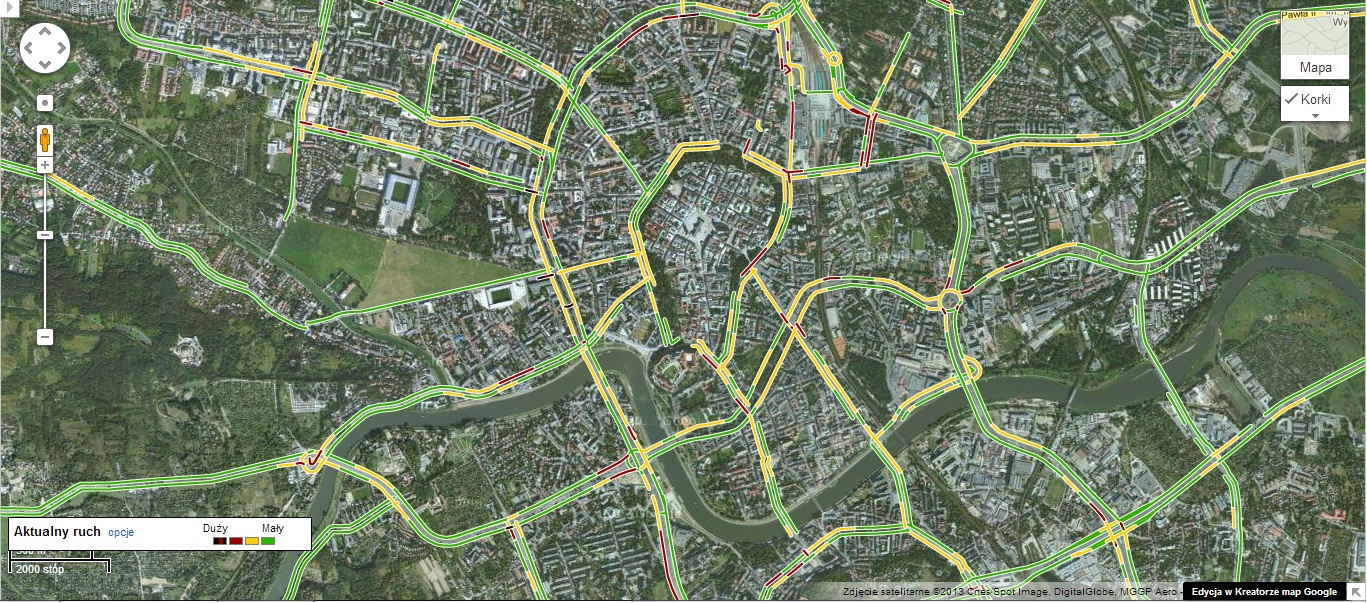
\includegraphics[width=100mm]{ge/gm_1.jpg}
  \caption{Google Maps.}
  \label{fig:googleMaps_1}
\end{figure}


\subsection{Windows Maps}
\label{subsec:Windows Maps}

Rysunek \ref{fig:bingMaps_1} przedstawia obraz otrzymany wykorzystując Bing Maps. W tym konkretnym przykładzie widzimy znaczną różnicę kolorów, obecność chmur pomniejsza wartość tych zdjęć. Należy wspomnieć o znacznie uboższym interfejsie dostarczanym użytkownikowi, interakcja jest w znacznym stopniu uboższa.

\begin{figure}[H]
  \centering
    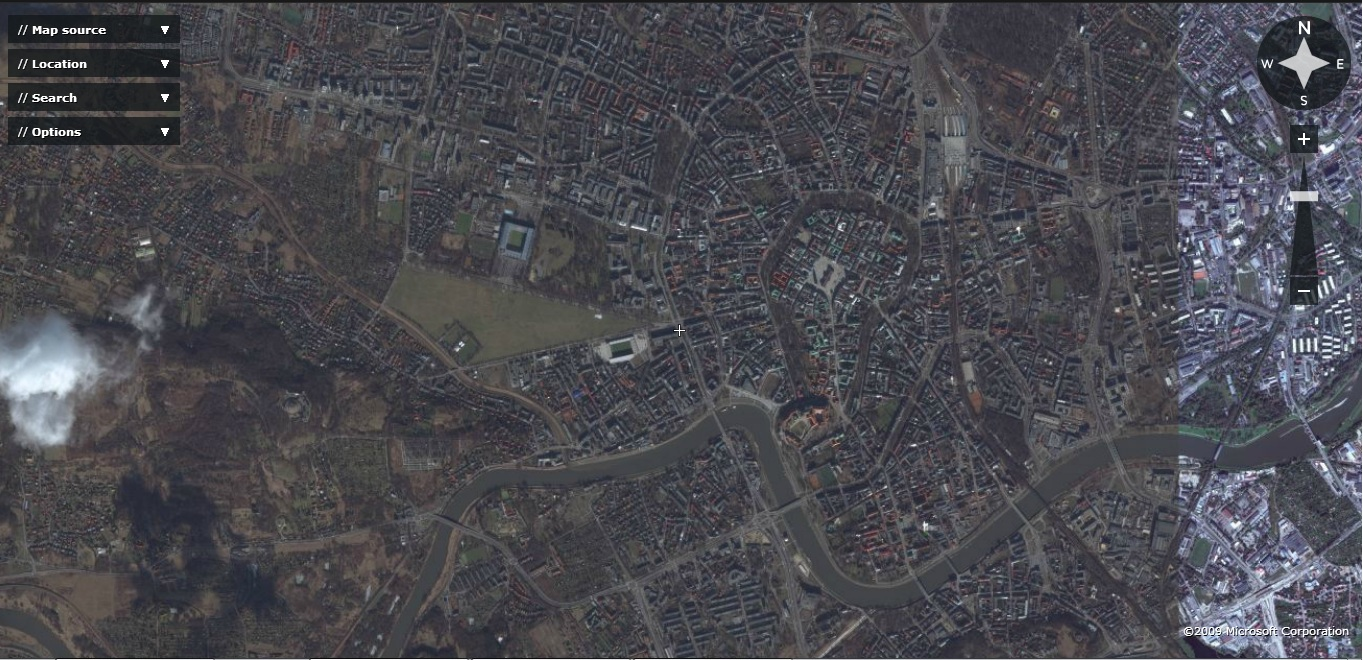
\includegraphics[width=100mm]{ge/bing_1.jpg}
  \caption{Bing Maps.}
  \label{fig:bingMaps_1}
\end{figure}

\subsection{Yahoo Maps}
\label{subsec:Yahoo Maps}

Kolejnym dostarczycielem danych kartograficznym jest Yahoo, przykład znajduje się na rysunku \ref{fig:yahooMaps_1}. Interfejs jest zbliżony do Bing Maps, jednak obszar na którym możemy przedlądać zdjęcia jest mniejszy, obszary oddalone od większych miast nie są w pełni uwzglęnione. Z tego powodu nie stanowi w pełni akceptowalnej alterantywy.

\begin{figure}[H]
  \centering
    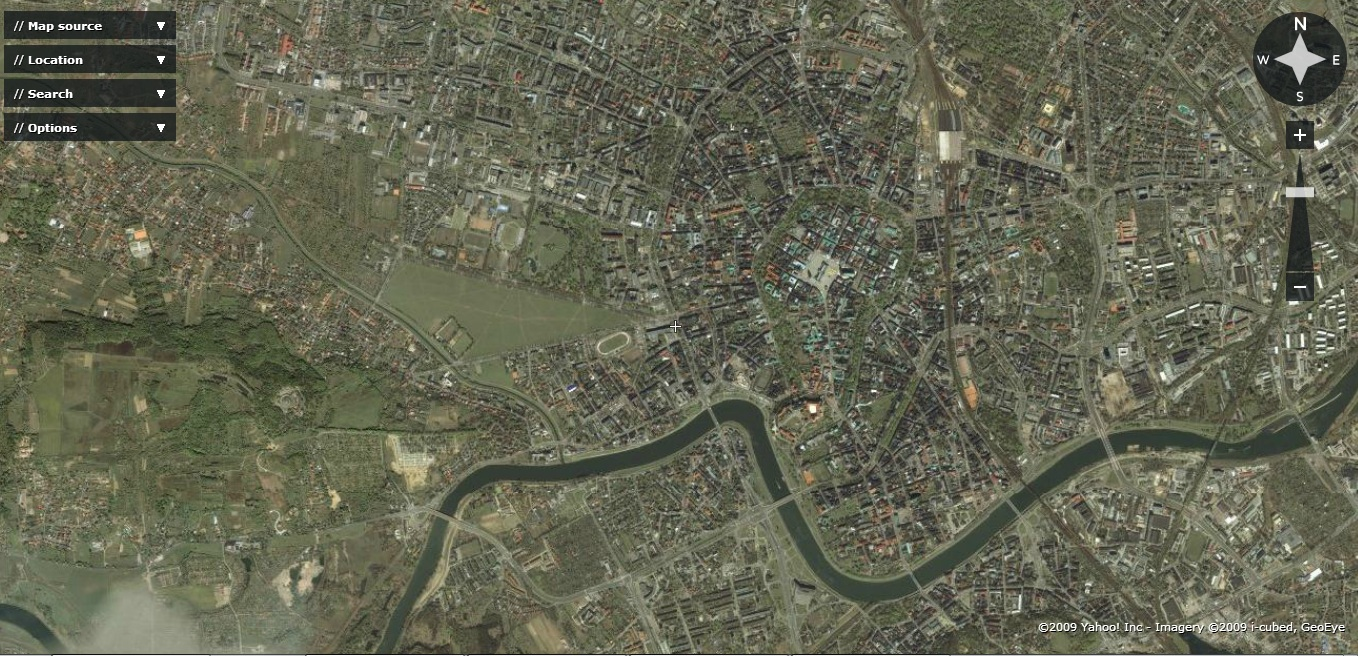
\includegraphics[width=100mm]{ge/yahoo_1.jpg}
  \caption{Yahoo Maps.}
  \label{fig:yahooMaps_1}
\end{figure}


\subsection{Apple Maps}
\label{subsec:Apple Maps}

Kolejną dużą marką która dostarcza informację jest Apple. Niestety nie ma wersji która pozwalałaby na dostęp do tej usługi z powszechnie używanych komputerów stacjonarnych. Dodatkowo jakość dostarczanych informacji jest bardzo złej jakości.



\section{Oś czasu}
\label{sec:osCzasu}

Jedną z większych uniedogonień podczas korzystania z map jest ich statyczność. Tradycyjne mapy pozwalają poznać jedynie jedną konkretną sytuację któa panowała na danym obszarze, nawet jeśli nałożymy kilka informacji z różnych okresów na jeden obraz, wynik może przestać być czytely. Korzystając w map dostępnych w internecie zazwyczaj istnieje opcja zmiany widoku. W jednej chwili możemy być na wysokości kilkuset kilometrów nad poziomem morza, aby w kolejnej znaleść się kilkaset metrów nad ziemią.

Ciekawą opcją jest dostarczana przez Google Earth możliwość zmiany czasu wykonania zdjęć. Niestety jest ona nieprzydatna jeśli chcemy przezentować własne dane.




